% ============================================================================
% MODERN PRACTICAL CONTROL SYSTEMS
% A Comprehensive Guide from Classical Theory to Machine Learning
% ============================================================================
% Author: J.C. Vaught
% Institution: University of South Carolina
% Molinaroli College of Engineering and Computing
% Department of Mechanical Engineering
% ============================================================================

\usepackage[utf8]{inputenc}
\usepackage[T1]{fontenc}
\usepackage{amsmath,amssymb,amsfonts,amsthm}
\usepackage{mathtools}
\usepackage{bm}
\usepackage{graphicx}
\usepackage{float}
\usepackage{subcaption}
\usepackage{booktabs}
\usepackage{array}
\usepackage{multirow}
\usepackage{longtable}
\usepackage{enumitem}
\usepackage{fancyhdr}
\usepackage{tikz}
\usepackage{pgfplots}
\usepackage{circuitikz}
\usepackage{siunitx}
\usepackage{hyperref}
\usepackage{cleveref}
\usepackage{xcolor}
\usepackage{tcolorbox}
\usepackage{algorithm}
\usepackage{algpseudocode}
\usepackage{listings}
\usepackage{geometry}
\usepackage{titlesec}
\usepackage{setspace}

% Page geometry
\geometry{
    letterpaper,
    margin=1in,
    headheight=14pt
}

% Paragraph formatting for lecture notes
\setlength{\parindent}{0pt}
\setlength{\parskip}{1ex plus 0.5ex minus 0.2ex}

% TikZ libraries
\usetikzlibrary{shapes,arrows,positioning,calc,patterns,decorations.pathmorphing,decorations.markings,circuits.ee.IEC,arrows.meta,bending}
\pgfplotsset{compat=1.18}

% ============================================================================
% UofSC Brand Color Palette
% ============================================================================
% Primary Colors
\definecolor{UofSCGarnet}{RGB}{115,0,10}
\definecolor{UofSCBlack}{RGB}{0,0,0}
\definecolor{UofSCWhite}{RGB}{255,255,255}
% Accent Colors
\definecolor{UofSCRose}{RGB}{204,46,64}
\definecolor{UofSCAtlantic}{RGB}{70,106,159}
\definecolor{UofSCCongaree}{RGB}{31,65,77}
\definecolor{UofSCHorseshoe}{RGB}{101,120,11}
\definecolor{UofSCGrass}{RGB}{206,211,24}
\definecolor{UofSCHoneycomb}{RGB}{164,145,55}
% Neutral Colors
\definecolor{UofSC90Black}{RGB}{54,54,54}
\definecolor{UofSC70Black}{RGB}{92,92,92}
\definecolor{UofSC50Black}{RGB}{162,162,162}
\definecolor{UofSCWarmGrey}{RGB}{103,97,86}
\definecolor{UofSCSandstorm}{RGB}{255,242,227}
% Special Colors
\definecolor{UofSCDarkGarnet}{RGB}{87,0,8}
\definecolor{UofSCAzalea}{RGB}{132,66,71}

% Semantic color aliases (for backwards compatibility and semantic use)
\definecolor{chaptercolor}{RGB}{115,0,10}      % UofSCGarnet for chapter titles
\definecolor{examplecolor}{RGB}{101,120,11}    % UofSCHorseshoe for examples
\definecolor{definitioncolor}{RGB}{70,106,159} % UofSCAtlantic for definitions
\definecolor{theoremcolor}{RGB}{87,0,8}        % UofSCDarkGarnet for theorems
\definecolor{warningcolor}{RGB}{204,46,64}     % UofSCRose for warnings
\definecolor{historicalcolor}{RGB}{103,97,86}  % UofSCWarmGrey for historical
\definecolor{codebackground}{RGB}{255,242,227} % UofSCSandstorm for code

% Theorem environments (numbered by section for lecture notes)
\theoremstyle{definition}
\newtheorem{definition}{Definition}[section]
\newtheorem{example}{Example}[section]
\newtheorem{exercise}{Exercise}[section]

\theoremstyle{plain}
\newtheorem{theorem}{Theorem}[section]
\newtheorem{lemma}[theorem]{Lemma}
\newtheorem{corollary}[theorem]{Corollary}
\newtheorem{proposition}[theorem]{Proposition}

\theoremstyle{remark}
\newtheorem{remark}{Remark}[section]
\newtheorem{note}{Note}[section]

% Custom tcolorbox environments
\tcbuselibrary{theorems,skins,breakable}

\newtcolorbox{keyconceptbox}[1][]{
    enhanced,
    colback=UofSCGarnet!5!white,
    colframe=UofSCGarnet,
    fonttitle=\bfseries,
    title=Key Concept,
    breakable,
    sharp corners,
    boxrule=1pt,
    #1
}

\newtcolorbox{warningbox}[1][]{
    enhanced,
    colback=UofSCRose!8!white,
    colframe=UofSCRose,
    fonttitle=\bfseries,
    title=Important Note,
    breakable,
    sharp corners,
    boxrule=1pt,
    #1
}

\newtcolorbox{examplebox}[1][]{
    enhanced,
    colback=UofSCHorseshoe!8!white,
    colframe=UofSCHorseshoe,
    fonttitle=\bfseries,
    breakable,
    sharp corners,
    boxrule=1pt,
    #1
}

\newtcolorbox{definitionbox}[1][]{
    enhanced,
    colback=UofSCAtlantic!8!white,
    colframe=UofSCAtlantic,
    fonttitle=\bfseries,
    breakable,
    sharp corners,
    boxrule=1pt,
    #1
}

\newtcolorbox{historicalbox}[1][]{
    enhanced,
    colback=UofSCSandstorm,
    colframe=UofSCWarmGrey,
    fonttitle=\bfseries,
    title=Historical Context,
    breakable,
    sharp corners,
    boxrule=1pt,
    #1
}

\newtcolorbox{practicalbox}[1][]{
    enhanced,
    colback=UofSCCongaree!8!white,
    colframe=UofSCCongaree,
    fonttitle=\bfseries,
    title=Practical Considerations,
    breakable,
    sharp corners,
    boxrule=1pt,
    #1
}

\newtcolorbox{matlabbox}[1][]{
    enhanced,
    colback=UofSCSandstorm,
    colframe=UofSC70Black,
    fonttitle=\bfseries\ttfamily,
    title=MATLAB/Python Code,
    breakable,
    sharp corners,
    boxrule=1pt,
    #1
}

% Code listing settings
\lstset{
    backgroundcolor=\color{codebackground},
    basicstyle=\ttfamily\small,
    breaklines=true,
    captionpos=b,
    commentstyle=\color{green!50!black},
    keywordstyle=\color{blue},
    stringstyle=\color{orange},
    numbers=left,
    numberstyle=\tiny\color{gray},
    frame=single,
    rulecolor=\color{black!30},
    tabsize=4
}

% Header and footer
\pagestyle{fancy}
\fancyhf{}
\fancyhead[LE,RO]{\thepage}
\fancyhead[RE]{\textit{\nouppercase{\leftmark}}}
\fancyhead[LO]{\textit{\nouppercase{\rightmark}}}
\renewcommand{\headrulewidth}{0.4pt}

% Custom commands for control systems
\newcommand{\Laplace}{\mathcal{L}}
\newcommand{\iLaplace}{\mathcal{L}^{-1}}
\newcommand{\Fourier}{\mathcal{F}}
\newcommand{\iFourier}{\mathcal{F}^{-1}}
\newcommand{\ZT}{\mathcal{Z}}
\newcommand{\iZT}{\mathcal{Z}^{-1}}
\newcommand{\Real}{\operatorname{Re}}
\newcommand{\Imag}{\operatorname{Im}}
\newcommand{\sgn}{\operatorname{sgn}}
\newcommand{\sinc}{\operatorname{sinc}}
\newcommand{\rect}{\operatorname{rect}}
\newcommand{\tri}{\operatorname{tri}}
\newcommand{\diag}{\operatorname{diag}}
\newcommand{\rank}{\operatorname{rank}}
\newcommand{\trace}{\operatorname{tr}}
\newcommand{\nullspace}{\operatorname{null}}
\newcommand{\range}{\operatorname{range}}
\newcommand{\vectornorm}[1]{\left\|#1\right\|}
\newcommand{\abs}[1]{\left|#1\right|}
\newcommand{\inner}[2]{\langle #1, #2 \rangle}
\newcommand{\dd}{\mathrm{d}}
\newcommand{\ee}{\mathrm{e}}
\newcommand{\ii}{\mathrm{i}}
\newcommand{\jj}{\mathrm{j}}
\newcommand{\TF}[2]{\frac{#1}{#2}}
\newcommand{\unitstep}{u(t)}
\newcommand{\impulse}{\delta(t)}
\newcommand{\conv}{\ast}

% Matrix shortcuts
\newcommand{\mA}{\mathbf{A}}
\newcommand{\mB}{\mathbf{B}}
\newcommand{\mC}{\mathbf{C}}
\newcommand{\mD}{\mathbf{D}}
\newcommand{\mE}{\mathbf{E}}
\newcommand{\mF}{\mathbf{F}}
\newcommand{\mG}{\mathbf{G}}
\newcommand{\mH}{\mathbf{H}}
\newcommand{\mI}{\mathbf{I}}
\newcommand{\mJ}{\mathbf{J}}
\newcommand{\mK}{\mathbf{K}}
\newcommand{\mL}{\mathbf{L}}
\newcommand{\mM}{\mathbf{M}}
\newcommand{\mN}{\mathbf{N}}
\newcommand{\mO}{\mathbf{O}}
\newcommand{\mP}{\mathbf{P}}
\newcommand{\mQ}{\mathbf{Q}}
\newcommand{\mR}{\mathbf{R}}
\newcommand{\mS}{\mathbf{S}}
\newcommand{\mT}{\mathbf{T}}
\newcommand{\mU}{\mathbf{U}}
\newcommand{\mV}{\mathbf{V}}
\newcommand{\mW}{\mathbf{W}}
\newcommand{\mX}{\mathbf{X}}
\newcommand{\mY}{\mathbf{Y}}
\newcommand{\mZ}{\mathbf{Z}}

% Vector shortcuts
\newcommand{\veca}{\mathbf{a}}
\newcommand{\vecb}{\mathbf{b}}
\newcommand{\vecc}{\mathbf{c}}
\newcommand{\vecd}{\mathbf{d}}
\newcommand{\vece}{\mathbf{e}}
\newcommand{\vecf}{\mathbf{f}}
\newcommand{\vecg}{\mathbf{g}}
\newcommand{\vech}{\mathbf{h}}
\newcommand{\veci}{\mathbf{i}}
\newcommand{\vecj}{\mathbf{j}}
\newcommand{\veck}{\mathbf{k}}
\newcommand{\vecl}{\mathbf{l}}
\newcommand{\vecm}{\mathbf{m}}
\newcommand{\vecn}{\mathbf{n}}
\newcommand{\veco}{\mathbf{o}}
\newcommand{\vecp}{\mathbf{p}}
\newcommand{\vecq}{\mathbf{q}}
\newcommand{\vecr}{\mathbf{r}}
\newcommand{\vecs}{\mathbf{s}}
\newcommand{\vect}{\mathbf{t}}
\newcommand{\vecu}{\mathbf{u}}
\newcommand{\vecv}{\mathbf{v}}
\newcommand{\vecw}{\mathbf{w}}
\newcommand{\vecx}{\mathbf{x}}
\newcommand{\vecy}{\mathbf{y}}
\newcommand{\vecz}{\mathbf{z}}

% SI unit shortcuts
\DeclareSIUnit\rpm{rpm}
\DeclareSIUnit\rad{rad}

% Block diagram styles (using UofSC colors, sharp corners)
\tikzset{
    block/.style={draw=UofSCBlack, fill=UofSCAtlantic!15, rectangle,
                  minimum height=2.5em, minimum width=4em, sharp corners,
                  font=\small},
    sumnode/.style={draw=UofSCBlack, circle, minimum size=1.2em,
                    inner sep=0pt, node distance=1.5cm},
    sum/.style={draw=UofSCBlack, circle, minimum size=1.2em,
                inner sep=0pt, node distance=1.5cm},
    input/.style={coordinate},
    output/.style={coordinate},
    pinstyle/.style={pin edge={to-,thin,black}},
    integrator/.style={draw=UofSCBlack, fill=UofSCHorseshoe!15, rectangle,
                       minimum height=2em, minimum width=2em, sharp corners},
    gain/.style={draw=UofSCBlack, fill=UofSCGarnet!15, isosceles triangle,
                 isosceles triangle apex angle=60, minimum height=1.5em, sharp corners},
    branch/.style={fill=UofSCBlack, shape=circle, minimum size=3pt, inner sep=0pt},
    plantblock/.style={draw=UofSCBlack, fill=UofSCCongaree!20, rectangle,
                       minimum height=2.5em, minimum width=4em, sharp corners,
                       font=\small},
    controllerblock/.style={draw=UofSCBlack, fill=UofSCGarnet!15, rectangle,
                            minimum height=2.5em, minimum width=4em, sharp corners,
                            font=\small},
    sensorblock/.style={draw=UofSCBlack, fill=UofSCHoneycomb!20, rectangle,
                        minimum height=2.5em, minimum width=4em, sharp corners,
                        font=\small},
    % Arrow styles
    signal/.style={->, >=stealth, thick},
    feedback/.style={->, >=stealth, thick}
}

% pgfplots color cycle using UofSC colors
\pgfplotscreateplotcyclelist{uofsc}{
    {UofSCGarnet, thick},
    {UofSCAtlantic, thick},
    {UofSCHorseshoe, thick},
    {UofSCCongaree, thick},
    {UofSCRose, thick},
    {UofSCHoneycomb, thick}
}

% Default pgfplots settings
\pgfplotsset{
    every axis/.append style={
        grid=major,
        grid style={UofSC50Black!30},
        tick style={UofSCBlack},
        label style={font=\small},
        legend style={font=\footnotesize, sharp corners, draw=UofSC70Black},
        cycle list name=uofsc
    }
}

% ============================================================================
% AUTHOR INFORMATION
% ============================================================================

\newcommand{\authorname}{J.C. Vaught}
\newcommand{\authorinstitution}{University of South Carolina}
\newcommand{\authordepartment}{Department of Mechanical Engineering}
\newcommand{\authorcollege}{Molinaroli College of Engineering and Computing}
\newcommand{\authorlocation}{Columbia, South Carolina}
\newcommand{\authoremail}{}
\newcommand{\textbooktitle}{Modern Practical Control Systems}
\newcommand{\textbooksubtitle}{From Classical Theory to Machine Learning}
\newcommand{\textbookversion}{1.0}
\newcommand{\textbookyear}{2026}

% ============================================================================
% TITLE PAGE COMMAND
% ============================================================================

\newcommand{\maketitlepage}{
    \begin{titlepage}
        \centering
        \vspace*{1.5cm}

        % Garnet rule at top
        {\color{UofSCGarnet}\rule{\textwidth}{3pt}}

        \vspace{1cm}

        {\Huge\bfseries\color{UofSCGarnet} \textbooktitle \par}
        \vspace{0.5cm}
        {\Large\itshape\color{UofSC70Black} \textbooksubtitle \par}

        \vspace{1.5cm}

        % Enhanced feedback control system diagram
        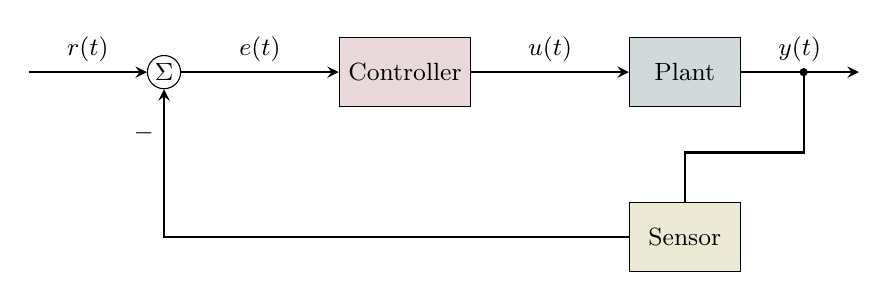
\begin{tikzpicture}[scale=0.85, node distance=2cm]
            % Nodes with UofSC styling
            \node[input] (input) {};
            \node[sum, right=of input, fill=white] (sum) {};
            \node[controllerblock, right=of sum] (controller) {Controller};
            \node[plantblock, right=of controller] (plant) {Plant};
            \coordinate[right=1.5cm of plant] (output);
            \node[sensorblock, below=1.2cm of plant] (sensor) {Sensor};

            % Sum node labels
            \node at (sum) {\small $\Sigma$};

            % Signal paths with arrows
            \draw[signal] (input) -- node[above, font=\small] {$r(t)$} (sum);
            \draw[signal] (sum) -- node[above, font=\small] {$e(t)$} (controller);
            \draw[signal] (controller) -- node[above, font=\small] {$u(t)$} (plant);
            \draw[signal] (plant) -- node[above, font=\small] {$y(t)$} (output);

            % Feedback path
            \coordinate[right=0.8cm of plant] (fb1);
            \draw[thick] (fb1) -- ++(0,-1.2) -| (sensor);
            \draw[signal] (sensor) -| node[left, pos=0.85, font=\small] {$-$} (sum);

            % Small dot at branch point
            \node[branch] at (fb1) {};
        \end{tikzpicture}

        \vspace{1.5cm}

        {\Large\bfseries \authorname \par}
        \vspace{0.4cm}
        {\large \authordepartment \par}
        \vspace{0.1cm}
        {\large \authorcollege \par}
        \vspace{0.1cm}
        {\large\color{UofSCGarnet} \authorinstitution \par}
        \vspace{0.1cm}
        {\large \authorlocation \par}

        \vfill

        % Bottom garnet rule
        {\color{UofSCGarnet}\rule{\textwidth}{3pt}}
        \vspace{0.3cm}
        {\large Version \textbookversion{} \hfill \textbookyear \par}
    \end{titlepage}
}

% ============================================================================
% ABOUT THE AUTHOR
% ============================================================================

\newcommand{\makeauthorpage}{
    \chapter*{About the Author}
    \addcontentsline{toc}{chapter}{About the Author}

    \textbf{J.C. Vaught} is a graduate researcher in the Department of Mechanical Engineering at the University of South Carolina, where he is pursuing his M.S. under the supervision of Dr. Yi Wang. His research interests span control systems, optimization algorithms, and the intersection of classical control theory with modern machine learning techniques.

    Throughout his academic career, Vaught has consistently demonstrated excellence, earning recognition on the President's List and Dean's List. His technical experience includes work on laser powder bed fusion additive manufacturing (LPBFAM) distortion prediction, CAD modeling, and finite element analysis.

    Beyond research, Vaught has shown exceptional leadership in engineering organizations. He served as President of both IEEE and SAE student chapters and as an advisor to ASME. Notably, he co-founded the University of South Carolina's first university-affiliated NAR-insured Rocketry Club, growing its membership from zero to over 120 students. He also served as Student Body Treasurer, successfully managing and expanding the student government budget.

    His diverse background in hands-on engineering, organizational leadership, and technical writing---including opinion contributions to \textit{The Daily Gamecock}---informs this textbook's practical approach to control systems education. This text reflects his belief that control theory should be accessible to students from all engineering disciplines while maintaining mathematical rigor.

    \vspace{1cm}

    \noindent\textit{For correspondence regarding this textbook, please contact the Department of Mechanical Engineering at the University of South Carolina.}
}

% ============================================================================
% PREFACE COMMAND
% ============================================================================

\newcommand{\makepreface}{
    \chapter*{Preface}
    \addcontentsline{toc}{chapter}{Preface}

    Control systems engineering stands at the intersection of mathematics, physics, and increasingly, computer science and artificial intelligence. From the thermostats in our homes to the autopilots in aircraft, from industrial robots to autonomous vehicles, control systems are ubiquitous in modern technology. This textbook aims to provide a comprehensive, practical introduction to control systems that bridges classical theory with contemporary machine learning approaches.

    \section*{Philosophy of This Text}

    This book is written with several guiding principles:

    \begin{enumerate}
        \item \textbf{Broad Applicability}: While many control systems texts focus primarily on electrical or mechanical systems, this book deliberately covers applications across mechanical, electrical, chemical, aerospace, civil, biomedical, industrial, and computer engineering. Each chapter includes diverse examples to help students see the universality of control concepts.

        \item \textbf{Mathematical Rigor with Intuition}: We begin with a comprehensive mathematical foundations chapter that reviews all prerequisite material---from complex numbers to linear algebra to probability theory. This ensures all students start from a common foundation while developing both computational skills and conceptual understanding.

        \item \textbf{Practical Focus}: Every theoretical concept is accompanied by worked examples, MATLAB/Python code, and real-world applications. Theory without application breeds confusion; application without theory breeds limitation.

        \item \textbf{Modern Integration}: This text seamlessly integrates classical control (Laplace transforms, root locus, Bode plots), modern control (state-space, optimal control), discrete-time control, and machine learning-based control (neural networks, reinforcement learning). Students learn when each approach is appropriate and how they complement each other.

        \item \textbf{Progressive Complexity}: We begin with ideal assumptions---perfect sensors, instantaneous actuators, linear dynamics---and progressively relax these to address real-world challenges. This scaffolded approach builds confidence before introducing complexity.
    \end{enumerate}

    \section*{How to Use This Book}

    The book is organized into several parts:

    \begin{itemize}
        \item \textbf{Part I: Foundations} covers mathematical prerequisites and system modeling with ideal components.

        \item \textbf{Part II: Classical Control} develops frequency-domain analysis and design techniques.

        \item \textbf{Part III: Modern Control} introduces state-space methods and optimal control.

        \item \textbf{Part IV: Discrete and Digital Control} addresses sampled-data systems and digital implementation.

        \item \textbf{Part V: Advanced Topics} covers nonlinear systems, robust control, and adaptive methods.

        \item \textbf{Part VI: Machine Learning in Control} explores neural networks, reinforcement learning, and hybrid approaches.
    \end{itemize}

    Each chapter includes learning objectives, worked examples, summary boxes, and end-of-chapter exercises ranging from computational to conceptual to design-oriented.

    \section*{Acknowledgments}

    I am grateful to Dr. Yi Wang for his mentorship and guidance throughout my graduate studies. Thanks also to the faculty and students of the Molinaroli College of Engineering and Computing who provided feedback on early drafts. The vibrant engineering community at the University of South Carolina---through organizations like IEEE, SAE, ASME, and the Rocketry Club---has continually inspired my belief in hands-on, practical engineering education.

    \vspace{1cm}

    \hfill J.C. Vaught

    \hfill Columbia, South Carolina

    \hfill \textbookyear
}
